% Created by tikzDevice version 0.8.1 on 2015-03-26 23:37:48
% !TEX encoding = UTF-8 Unicode
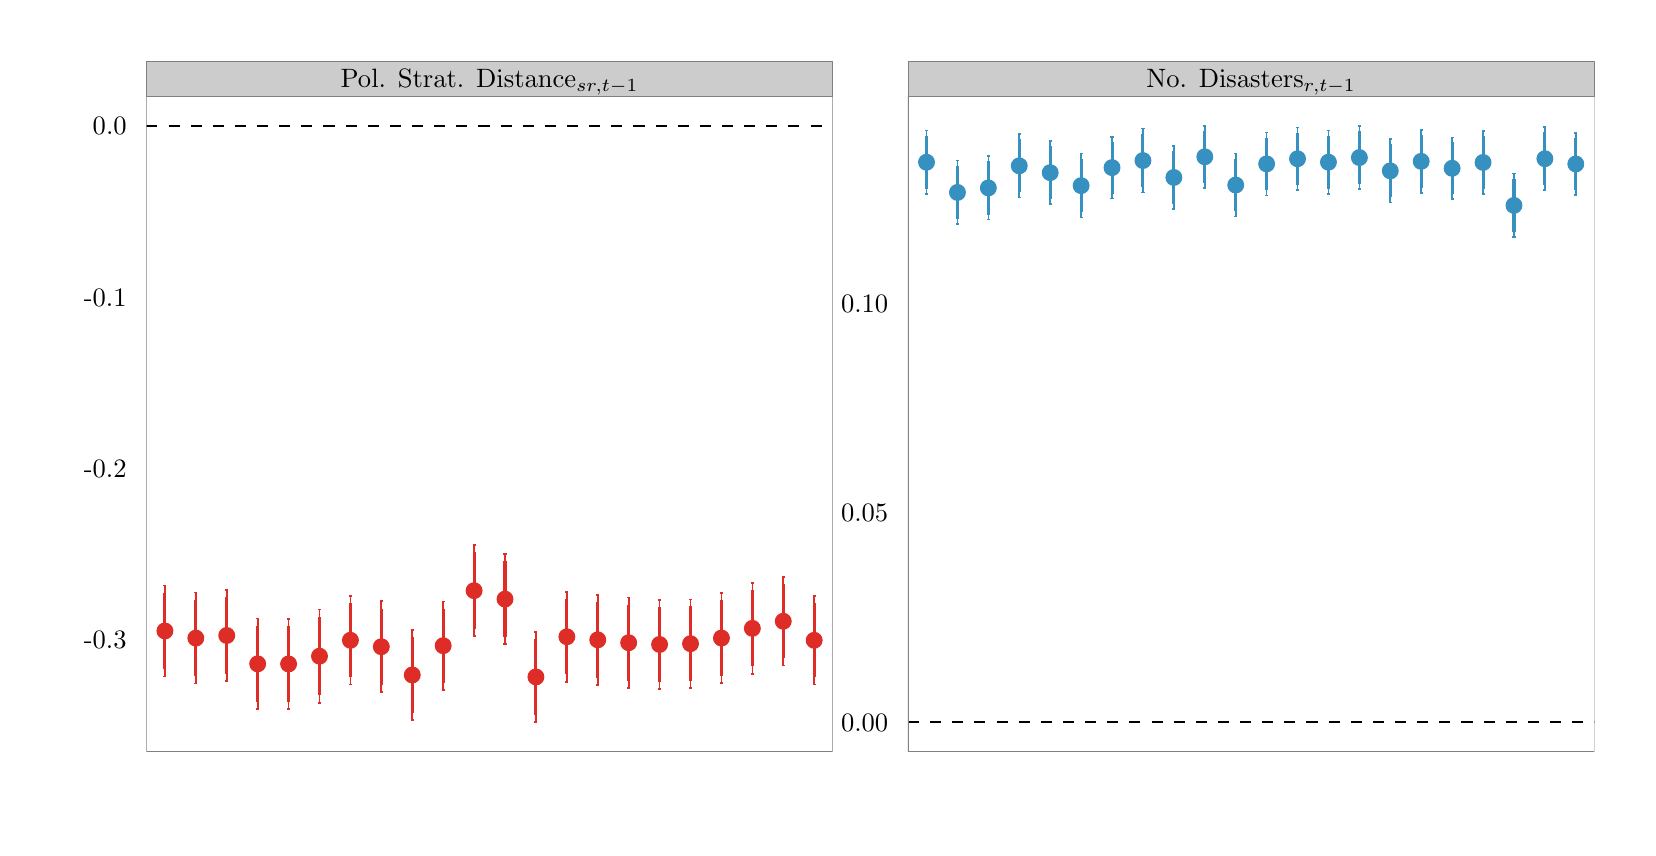
\begin{tikzpicture}[x=1pt,y=1pt]
\definecolor{fillColor}{RGB}{255,255,255}
\path[use as bounding box,fill=fillColor,fill opacity=0.00] (0,0) rectangle (578.16,289.08);
\begin{scope}
\path[clip] (  0.00,  0.00) rectangle (578.16,289.08);
\definecolor{drawColor}{RGB}{255,255,255}
\definecolor{fillColor}{RGB}{255,255,255}

\path[draw=drawColor,line width= 0.6pt,line join=round,line cap=round,fill=fillColor] (  0.00,  0.00) rectangle (578.16,289.08);
\end{scope}
\begin{scope}
\path[clip] ( 42.89, 27.42) rectangle (290.91,264.40);
\definecolor{fillColor}{RGB}{255,255,255}

\path[fill=fillColor] ( 42.89, 27.42) rectangle (290.91,264.40);
\definecolor{drawColor}{RGB}{222,45,38}

\path[draw=drawColor,draw opacity=0.30,line width= 0.3pt,line join=round] ( 49.59, 54.65) -- ( 49.59, 87.54);

\path[draw=drawColor,draw opacity=0.30,line width= 0.3pt,line join=round] ( 60.76, 52.06) -- ( 60.76, 84.94);

\path[draw=drawColor,draw opacity=0.30,line width= 0.3pt,line join=round] ( 71.93, 52.97) -- ( 71.93, 85.93);

\path[draw=drawColor,draw opacity=0.30,line width= 0.3pt,line join=round] ( 83.11, 42.79) -- ( 83.11, 75.61);

\path[draw=drawColor,draw opacity=0.30,line width= 0.3pt,line join=round] ( 94.28, 42.85) -- ( 94.28, 75.47);

\path[draw=drawColor,draw opacity=0.30,line width= 0.3pt,line join=round] (105.45, 45.15) -- (105.45, 78.78);

\path[draw=drawColor,draw opacity=0.30,line width= 0.3pt,line join=round] (116.62, 51.70) -- (116.62, 83.72);

\path[draw=drawColor,draw opacity=0.30,line width= 0.3pt,line join=round] (127.79, 48.99) -- (127.79, 81.79);

\path[draw=drawColor,draw opacity=0.30,line width= 0.3pt,line join=round] (138.97, 38.93) -- (138.97, 71.43);

\path[draw=drawColor,draw opacity=0.30,line width= 0.3pt,line join=round] (150.14, 49.76) -- (150.14, 81.76);

\path[draw=drawColor,draw opacity=0.30,line width= 0.3pt,line join=round] (161.31, 69.15) -- (161.31,102.13);

\path[draw=drawColor,draw opacity=0.30,line width= 0.3pt,line join=round] (172.48, 66.38) -- (172.48, 98.79);

\path[draw=drawColor,draw opacity=0.30,line width= 0.3pt,line join=round] (183.65, 38.19) -- (183.65, 70.75);

\path[draw=drawColor,draw opacity=0.30,line width= 0.3pt,line join=round] (194.83, 52.74) -- (194.83, 85.24);

\path[draw=drawColor,draw opacity=0.30,line width= 0.3pt,line join=round] (206.00, 51.64) -- (206.00, 84.10);

\path[draw=drawColor,draw opacity=0.30,line width= 0.3pt,line join=round] (217.17, 50.45) -- (217.17, 83.21);

\path[draw=drawColor,draw opacity=0.30,line width= 0.3pt,line join=round] (228.34, 50.13) -- (228.34, 82.28);

\path[draw=drawColor,draw opacity=0.30,line width= 0.3pt,line join=round] (239.52, 50.47) -- (239.52, 82.50);

\path[draw=drawColor,draw opacity=0.30,line width= 0.3pt,line join=round] (250.69, 52.33) -- (250.69, 84.70);

\path[draw=drawColor,draw opacity=0.30,line width= 0.3pt,line join=round] (261.86, 55.60) -- (261.86, 88.45);

\path[draw=drawColor,draw opacity=0.30,line width= 0.3pt,line join=round] (273.03, 58.57) -- (273.03, 90.61);

\path[draw=drawColor,draw opacity=0.30,line width= 0.3pt,line join=round] (284.20, 51.73) -- (284.20, 83.68);
\definecolor{drawColor}{RGB}{222,45,38}

\path[draw=drawColor,line width= 1.1pt,line join=round] ( 49.59, 57.29) -- ( 49.59, 84.90);

\path[draw=drawColor,line width= 1.1pt,line join=round] ( 60.76, 54.70) -- ( 60.76, 82.30);

\path[draw=drawColor,line width= 1.1pt,line join=round] ( 71.93, 55.62) -- ( 71.93, 83.28);

\path[draw=drawColor,line width= 1.1pt,line join=round] ( 83.11, 45.43) -- ( 83.11, 72.97);

\path[draw=drawColor,line width= 1.1pt,line join=round] ( 94.28, 45.47) -- ( 94.28, 72.85);

\path[draw=drawColor,line width= 1.1pt,line join=round] (105.45, 47.85) -- (105.45, 76.08);

\path[draw=drawColor,line width= 1.1pt,line join=round] (116.62, 54.28) -- (116.62, 81.14);

\path[draw=drawColor,line width= 1.1pt,line join=round] (127.79, 51.63) -- (127.79, 79.15);

\path[draw=drawColor,line width= 1.1pt,line join=round] (138.97, 41.54) -- (138.97, 68.82);

\path[draw=drawColor,line width= 1.1pt,line join=round] (150.14, 52.33) -- (150.14, 79.19);

\path[draw=drawColor,line width= 1.1pt,line join=round] (161.31, 71.80) -- (161.31, 99.48);

\path[draw=drawColor,line width= 1.1pt,line join=round] (172.48, 68.99) -- (172.48, 96.19);

\path[draw=drawColor,line width= 1.1pt,line join=round] (183.65, 40.81) -- (183.65, 68.13);

\path[draw=drawColor,line width= 1.1pt,line join=round] (194.83, 55.35) -- (194.83, 82.63);

\path[draw=drawColor,line width= 1.1pt,line join=round] (206.00, 54.25) -- (206.00, 81.49);

\path[draw=drawColor,line width= 1.1pt,line join=round] (217.17, 53.08) -- (217.17, 80.57);

\path[draw=drawColor,line width= 1.1pt,line join=round] (228.34, 52.72) -- (228.34, 79.69);

\path[draw=drawColor,line width= 1.1pt,line join=round] (239.52, 53.05) -- (239.52, 79.92);

\path[draw=drawColor,line width= 1.1pt,line join=round] (250.69, 54.93) -- (250.69, 82.10);

\path[draw=drawColor,line width= 1.1pt,line join=round] (261.86, 58.24) -- (261.86, 85.81);

\path[draw=drawColor,line width= 1.1pt,line join=round] (273.03, 61.14) -- (273.03, 88.04);

\path[draw=drawColor,line width= 1.1pt,line join=round] (284.20, 54.30) -- (284.20, 81.11);
\definecolor{drawColor}{RGB}{0,0,0}

\path[draw=drawColor,line width= 0.6pt,dash pattern=on 4pt off 4pt ,line join=round] ( 42.89,253.63) -- (290.91,253.63);
\definecolor{drawColor}{RGB}{222,45,38}
\definecolor{fillColor}{RGB}{222,45,38}

\path[draw=drawColor,line width= 0.4pt,line join=round,line cap=round,fill=fillColor] ( 49.59, 71.09) circle (  2.85);

\path[draw=drawColor,line width= 0.4pt,line join=round,line cap=round,fill=fillColor] ( 60.76, 68.50) circle (  2.85);

\path[draw=drawColor,line width= 0.4pt,line join=round,line cap=round,fill=fillColor] ( 71.93, 69.45) circle (  2.85);

\path[draw=drawColor,line width= 0.4pt,line join=round,line cap=round,fill=fillColor] ( 83.11, 59.20) circle (  2.85);

\path[draw=drawColor,line width= 0.4pt,line join=round,line cap=round,fill=fillColor] ( 94.28, 59.16) circle (  2.85);

\path[draw=drawColor,line width= 0.4pt,line join=round,line cap=round,fill=fillColor] (105.45, 61.97) circle (  2.85);

\path[draw=drawColor,line width= 0.4pt,line join=round,line cap=round,fill=fillColor] (116.62, 67.71) circle (  2.85);

\path[draw=drawColor,line width= 0.4pt,line join=round,line cap=round,fill=fillColor] (127.79, 65.39) circle (  2.85);

\path[draw=drawColor,line width= 0.4pt,line join=round,line cap=round,fill=fillColor] (138.97, 55.18) circle (  2.85);

\path[draw=drawColor,line width= 0.4pt,line join=round,line cap=round,fill=fillColor] (150.14, 65.76) circle (  2.85);

\path[draw=drawColor,line width= 0.4pt,line join=round,line cap=round,fill=fillColor] (161.31, 85.64) circle (  2.85);

\path[draw=drawColor,line width= 0.4pt,line join=round,line cap=round,fill=fillColor] (172.48, 82.59) circle (  2.85);

\path[draw=drawColor,line width= 0.4pt,line join=round,line cap=round,fill=fillColor] (183.65, 54.47) circle (  2.85);

\path[draw=drawColor,line width= 0.4pt,line join=round,line cap=round,fill=fillColor] (194.83, 68.99) circle (  2.85);

\path[draw=drawColor,line width= 0.4pt,line join=round,line cap=round,fill=fillColor] (206.00, 67.87) circle (  2.85);

\path[draw=drawColor,line width= 0.4pt,line join=round,line cap=round,fill=fillColor] (217.17, 66.83) circle (  2.85);

\path[draw=drawColor,line width= 0.4pt,line join=round,line cap=round,fill=fillColor] (228.34, 66.20) circle (  2.85);

\path[draw=drawColor,line width= 0.4pt,line join=round,line cap=round,fill=fillColor] (239.52, 66.49) circle (  2.85);

\path[draw=drawColor,line width= 0.4pt,line join=round,line cap=round,fill=fillColor] (250.69, 68.51) circle (  2.85);

\path[draw=drawColor,line width= 0.4pt,line join=round,line cap=round,fill=fillColor] (261.86, 72.03) circle (  2.85);

\path[draw=drawColor,line width= 0.4pt,line join=round,line cap=round,fill=fillColor] (273.03, 74.59) circle (  2.85);

\path[draw=drawColor,line width= 0.4pt,line join=round,line cap=round,fill=fillColor] (284.20, 67.70) circle (  2.85);

\path[draw=drawColor,line width= 0.6pt,line join=round] ( 49.03, 87.54) --
	( 50.15, 87.54);

\path[draw=drawColor,line width= 0.6pt,line join=round] ( 49.59, 87.54) --
	( 49.59, 54.65);

\path[draw=drawColor,line width= 0.6pt,line join=round] ( 49.03, 54.65) --
	( 50.15, 54.65);

\path[draw=drawColor,line width= 0.6pt,line join=round] ( 60.20, 84.94) --
	( 61.32, 84.94);

\path[draw=drawColor,line width= 0.6pt,line join=round] ( 60.76, 84.94) --
	( 60.76, 52.06);

\path[draw=drawColor,line width= 0.6pt,line join=round] ( 60.20, 52.06) --
	( 61.32, 52.06);

\path[draw=drawColor,line width= 0.6pt,line join=round] ( 71.37, 85.93) --
	( 72.49, 85.93);

\path[draw=drawColor,line width= 0.6pt,line join=round] ( 71.93, 85.93) --
	( 71.93, 52.97);

\path[draw=drawColor,line width= 0.6pt,line join=round] ( 71.37, 52.97) --
	( 72.49, 52.97);

\path[draw=drawColor,line width= 0.6pt,line join=round] ( 82.55, 75.61) --
	( 83.66, 75.61);

\path[draw=drawColor,line width= 0.6pt,line join=round] ( 83.11, 75.61) --
	( 83.11, 42.79);

\path[draw=drawColor,line width= 0.6pt,line join=round] ( 82.55, 42.79) --
	( 83.66, 42.79);

\path[draw=drawColor,line width= 0.6pt,line join=round] ( 93.72, 75.47) --
	( 94.84, 75.47);

\path[draw=drawColor,line width= 0.6pt,line join=round] ( 94.28, 75.47) --
	( 94.28, 42.85);

\path[draw=drawColor,line width= 0.6pt,line join=round] ( 93.72, 42.85) --
	( 94.84, 42.85);

\path[draw=drawColor,line width= 0.6pt,line join=round] (104.89, 78.78) --
	(106.01, 78.78);

\path[draw=drawColor,line width= 0.6pt,line join=round] (105.45, 78.78) --
	(105.45, 45.15);

\path[draw=drawColor,line width= 0.6pt,line join=round] (104.89, 45.15) --
	(106.01, 45.15);

\path[draw=drawColor,line width= 0.6pt,line join=round] (116.06, 83.72) --
	(117.18, 83.72);

\path[draw=drawColor,line width= 0.6pt,line join=round] (116.62, 83.72) --
	(116.62, 51.70);

\path[draw=drawColor,line width= 0.6pt,line join=round] (116.06, 51.70) --
	(117.18, 51.70);

\path[draw=drawColor,line width= 0.6pt,line join=round] (127.24, 81.79) --
	(128.35, 81.79);

\path[draw=drawColor,line width= 0.6pt,line join=round] (127.79, 81.79) --
	(127.79, 48.99);

\path[draw=drawColor,line width= 0.6pt,line join=round] (127.24, 48.99) --
	(128.35, 48.99);

\path[draw=drawColor,line width= 0.6pt,line join=round] (138.41, 71.43) --
	(139.52, 71.43);

\path[draw=drawColor,line width= 0.6pt,line join=round] (138.97, 71.43) --
	(138.97, 38.93);

\path[draw=drawColor,line width= 0.6pt,line join=round] (138.41, 38.93) --
	(139.52, 38.93);

\path[draw=drawColor,line width= 0.6pt,line join=round] (149.58, 81.76) --
	(150.70, 81.76);

\path[draw=drawColor,line width= 0.6pt,line join=round] (150.14, 81.76) --
	(150.14, 49.76);

\path[draw=drawColor,line width= 0.6pt,line join=round] (149.58, 49.76) --
	(150.70, 49.76);

\path[draw=drawColor,line width= 0.6pt,line join=round] (160.75,102.13) --
	(161.87,102.13);

\path[draw=drawColor,line width= 0.6pt,line join=round] (161.31,102.13) --
	(161.31, 69.15);

\path[draw=drawColor,line width= 0.6pt,line join=round] (160.75, 69.15) --
	(161.87, 69.15);

\path[draw=drawColor,line width= 0.6pt,line join=round] (171.92, 98.79) --
	(173.04, 98.79);

\path[draw=drawColor,line width= 0.6pt,line join=round] (172.48, 98.79) --
	(172.48, 66.38);

\path[draw=drawColor,line width= 0.6pt,line join=round] (171.92, 66.38) --
	(173.04, 66.38);

\path[draw=drawColor,line width= 0.6pt,line join=round] (183.10, 70.75) --
	(184.21, 70.75);

\path[draw=drawColor,line width= 0.6pt,line join=round] (183.65, 70.75) --
	(183.65, 38.19);

\path[draw=drawColor,line width= 0.6pt,line join=round] (183.10, 38.19) --
	(184.21, 38.19);

\path[draw=drawColor,line width= 0.6pt,line join=round] (194.27, 85.24) --
	(195.39, 85.24);

\path[draw=drawColor,line width= 0.6pt,line join=round] (194.83, 85.24) --
	(194.83, 52.74);

\path[draw=drawColor,line width= 0.6pt,line join=round] (194.27, 52.74) --
	(195.39, 52.74);

\path[draw=drawColor,line width= 0.6pt,line join=round] (205.44, 84.10) --
	(206.56, 84.10);

\path[draw=drawColor,line width= 0.6pt,line join=round] (206.00, 84.10) --
	(206.00, 51.64);

\path[draw=drawColor,line width= 0.6pt,line join=round] (205.44, 51.64) --
	(206.56, 51.64);

\path[draw=drawColor,line width= 0.6pt,line join=round] (216.61, 83.21) --
	(217.73, 83.21);

\path[draw=drawColor,line width= 0.6pt,line join=round] (217.17, 83.21) --
	(217.17, 50.45);

\path[draw=drawColor,line width= 0.6pt,line join=round] (216.61, 50.45) --
	(217.73, 50.45);

\path[draw=drawColor,line width= 0.6pt,line join=round] (227.78, 82.28) --
	(228.90, 82.28);

\path[draw=drawColor,line width= 0.6pt,line join=round] (228.34, 82.28) --
	(228.34, 50.13);

\path[draw=drawColor,line width= 0.6pt,line join=round] (227.78, 50.13) --
	(228.90, 50.13);

\path[draw=drawColor,line width= 0.6pt,line join=round] (238.96, 82.50) --
	(240.07, 82.50);

\path[draw=drawColor,line width= 0.6pt,line join=round] (239.52, 82.50) --
	(239.52, 50.47);

\path[draw=drawColor,line width= 0.6pt,line join=round] (238.96, 50.47) --
	(240.07, 50.47);

\path[draw=drawColor,line width= 0.6pt,line join=round] (250.13, 84.70) --
	(251.25, 84.70);

\path[draw=drawColor,line width= 0.6pt,line join=round] (250.69, 84.70) --
	(250.69, 52.33);

\path[draw=drawColor,line width= 0.6pt,line join=round] (250.13, 52.33) --
	(251.25, 52.33);

\path[draw=drawColor,line width= 0.6pt,line join=round] (261.30, 88.45) --
	(262.42, 88.45);

\path[draw=drawColor,line width= 0.6pt,line join=round] (261.86, 88.45) --
	(261.86, 55.60);

\path[draw=drawColor,line width= 0.6pt,line join=round] (261.30, 55.60) --
	(262.42, 55.60);

\path[draw=drawColor,line width= 0.6pt,line join=round] (272.47, 90.61) --
	(273.59, 90.61);

\path[draw=drawColor,line width= 0.6pt,line join=round] (273.03, 90.61) --
	(273.03, 58.57);

\path[draw=drawColor,line width= 0.6pt,line join=round] (272.47, 58.57) --
	(273.59, 58.57);

\path[draw=drawColor,line width= 0.6pt,line join=round] (283.65, 83.68) --
	(284.76, 83.68);

\path[draw=drawColor,line width= 0.6pt,line join=round] (284.20, 83.68) --
	(284.20, 51.73);

\path[draw=drawColor,line width= 0.6pt,line join=round] (283.65, 51.73) --
	(284.76, 51.73);
\definecolor{drawColor}{gray}{0.50}

\path[draw=drawColor,line width= 0.6pt,line join=round,line cap=round] ( 42.89, 27.42) rectangle (290.91,264.40);
\end{scope}
\begin{scope}
\path[clip] (318.09, 27.42) rectangle (566.12,264.40);
\definecolor{fillColor}{RGB}{255,255,255}

\path[fill=fillColor] (318.09, 27.42) rectangle (566.12,264.40);
\definecolor{drawColor}{RGB}{54,144,192}

\path[draw=drawColor,draw opacity=0.30,line width= 0.3pt,line join=round] (324.80,228.95) -- (324.80,251.94);

\path[draw=drawColor,draw opacity=0.30,line width= 0.3pt,line join=round] (335.97,218.04) -- (335.97,241.04);

\path[draw=drawColor,draw opacity=0.30,line width= 0.3pt,line join=round] (347.14,219.70) -- (347.14,242.63);

\path[draw=drawColor,draw opacity=0.30,line width= 0.3pt,line join=round] (358.31,227.71) -- (358.31,250.59);

\path[draw=drawColor,draw opacity=0.30,line width= 0.3pt,line join=round] (369.49,225.30) -- (369.49,248.09);

\path[draw=drawColor,draw opacity=0.30,line width= 0.3pt,line join=round] (380.66,220.43) -- (380.66,243.57);

\path[draw=drawColor,draw opacity=0.30,line width= 0.3pt,line join=round] (391.83,227.34) -- (391.83,249.69);

\path[draw=drawColor,draw opacity=0.30,line width= 0.3pt,line join=round] (403.00,229.51) -- (403.00,252.60);

\path[draw=drawColor,draw opacity=0.30,line width= 0.3pt,line join=round] (414.17,223.62) -- (414.17,246.28);

\path[draw=drawColor,draw opacity=0.30,line width= 0.3pt,line join=round] (425.35,231.23) -- (425.35,253.63);

\path[draw=drawColor,draw opacity=0.30,line width= 0.3pt,line join=round] (436.52,220.82) -- (436.52,243.62);

\path[draw=drawColor,draw opacity=0.30,line width= 0.3pt,line join=round] (447.69,228.49) -- (447.69,251.22);

\path[draw=drawColor,draw opacity=0.30,line width= 0.3pt,line join=round] (458.86,230.39) -- (458.86,253.00);

\path[draw=drawColor,draw opacity=0.30,line width= 0.3pt,line join=round] (470.03,229.07) -- (470.03,251.88);

\path[draw=drawColor,draw opacity=0.30,line width= 0.3pt,line join=round] (481.21,230.72) -- (481.21,253.56);

\path[draw=drawColor,draw opacity=0.30,line width= 0.3pt,line join=round] (492.38,225.87) -- (492.38,248.80);

\path[draw=drawColor,draw opacity=0.30,line width= 0.3pt,line join=round] (503.55,229.40) -- (503.55,252.14);

\path[draw=drawColor,draw opacity=0.30,line width= 0.3pt,line join=round] (514.72,227.08) -- (514.72,249.45);

\path[draw=drawColor,draw opacity=0.30,line width= 0.3pt,line join=round] (525.90,229.07) -- (525.90,251.67);

\path[draw=drawColor,draw opacity=0.30,line width= 0.3pt,line join=round] (537.07,213.36) -- (537.07,236.34);

\path[draw=drawColor,draw opacity=0.30,line width= 0.3pt,line join=round] (548.24,230.36) -- (548.24,253.08);

\path[draw=drawColor,draw opacity=0.30,line width= 0.3pt,line join=round] (559.41,228.58) -- (559.41,251.09);
\definecolor{drawColor}{RGB}{54,144,192}

\path[draw=drawColor,line width= 1.1pt,line join=round] (324.80,230.80) -- (324.80,250.09);

\path[draw=drawColor,line width= 1.1pt,line join=round] (335.97,219.89) -- (335.97,239.19);

\path[draw=drawColor,line width= 1.1pt,line join=round] (347.14,221.55) -- (347.14,240.78);

\path[draw=drawColor,line width= 1.1pt,line join=round] (358.31,229.55) -- (358.31,248.75);

\path[draw=drawColor,line width= 1.1pt,line join=round] (369.49,227.13) -- (369.49,246.26);

\path[draw=drawColor,line width= 1.1pt,line join=round] (380.66,222.29) -- (380.66,241.71);

\path[draw=drawColor,line width= 1.1pt,line join=round] (391.83,229.14) -- (391.83,247.89);

\path[draw=drawColor,line width= 1.1pt,line join=round] (403.00,231.37) -- (403.00,250.74);

\path[draw=drawColor,line width= 1.1pt,line join=round] (414.17,225.44) -- (414.17,244.46);

\path[draw=drawColor,line width= 1.1pt,line join=round] (425.35,233.04) -- (425.35,251.83);

\path[draw=drawColor,line width= 1.1pt,line join=round] (436.52,222.66) -- (436.52,241.79);

\path[draw=drawColor,line width= 1.1pt,line join=round] (447.69,230.32) -- (447.69,249.39);

\path[draw=drawColor,line width= 1.1pt,line join=round] (458.86,232.21) -- (458.86,251.19);

\path[draw=drawColor,line width= 1.1pt,line join=round] (470.03,230.90) -- (470.03,250.05);

\path[draw=drawColor,line width= 1.1pt,line join=round] (481.21,232.56) -- (481.21,251.73);

\path[draw=drawColor,line width= 1.1pt,line join=round] (492.38,227.72) -- (492.38,246.96);

\path[draw=drawColor,line width= 1.1pt,line join=round] (503.55,231.23) -- (503.55,250.31);

\path[draw=drawColor,line width= 1.1pt,line join=round] (514.72,228.88) -- (514.72,247.65);

\path[draw=drawColor,line width= 1.1pt,line join=round] (525.90,230.89) -- (525.90,249.85);

\path[draw=drawColor,line width= 1.1pt,line join=round] (537.07,215.21) -- (537.07,234.49);

\path[draw=drawColor,line width= 1.1pt,line join=round] (548.24,232.19) -- (548.24,251.25);

\path[draw=drawColor,line width= 1.1pt,line join=round] (559.41,230.39) -- (559.41,249.28);
\definecolor{drawColor}{RGB}{0,0,0}

\path[draw=drawColor,line width= 0.6pt,dash pattern=on 4pt off 4pt ,line join=round] (318.09, 38.19) -- (566.12, 38.19);
\definecolor{drawColor}{RGB}{54,144,192}
\definecolor{fillColor}{RGB}{54,144,192}

\path[draw=drawColor,line width= 0.4pt,line join=round,line cap=round,fill=fillColor] (324.80,240.45) circle (  2.85);

\path[draw=drawColor,line width= 0.4pt,line join=round,line cap=round,fill=fillColor] (335.97,229.54) circle (  2.85);

\path[draw=drawColor,line width= 0.4pt,line join=round,line cap=round,fill=fillColor] (347.14,231.17) circle (  2.85);

\path[draw=drawColor,line width= 0.4pt,line join=round,line cap=round,fill=fillColor] (358.31,239.15) circle (  2.85);

\path[draw=drawColor,line width= 0.4pt,line join=round,line cap=round,fill=fillColor] (369.49,236.69) circle (  2.85);

\path[draw=drawColor,line width= 0.4pt,line join=round,line cap=round,fill=fillColor] (380.66,232.00) circle (  2.85);

\path[draw=drawColor,line width= 0.4pt,line join=round,line cap=round,fill=fillColor] (391.83,238.51) circle (  2.85);

\path[draw=drawColor,line width= 0.4pt,line join=round,line cap=round,fill=fillColor] (403.00,241.06) circle (  2.85);

\path[draw=drawColor,line width= 0.4pt,line join=round,line cap=round,fill=fillColor] (414.17,234.95) circle (  2.85);

\path[draw=drawColor,line width= 0.4pt,line join=round,line cap=round,fill=fillColor] (425.35,242.43) circle (  2.85);

\path[draw=drawColor,line width= 0.4pt,line join=round,line cap=round,fill=fillColor] (436.52,232.22) circle (  2.85);

\path[draw=drawColor,line width= 0.4pt,line join=round,line cap=round,fill=fillColor] (447.69,239.86) circle (  2.85);

\path[draw=drawColor,line width= 0.4pt,line join=round,line cap=round,fill=fillColor] (458.86,241.70) circle (  2.85);

\path[draw=drawColor,line width= 0.4pt,line join=round,line cap=round,fill=fillColor] (470.03,240.47) circle (  2.85);

\path[draw=drawColor,line width= 0.4pt,line join=round,line cap=round,fill=fillColor] (481.21,242.14) circle (  2.85);

\path[draw=drawColor,line width= 0.4pt,line join=round,line cap=round,fill=fillColor] (492.38,237.34) circle (  2.85);

\path[draw=drawColor,line width= 0.4pt,line join=round,line cap=round,fill=fillColor] (503.55,240.77) circle (  2.85);

\path[draw=drawColor,line width= 0.4pt,line join=round,line cap=round,fill=fillColor] (514.72,238.26) circle (  2.85);

\path[draw=drawColor,line width= 0.4pt,line join=round,line cap=round,fill=fillColor] (525.90,240.37) circle (  2.85);

\path[draw=drawColor,line width= 0.4pt,line join=round,line cap=round,fill=fillColor] (537.07,224.85) circle (  2.85);

\path[draw=drawColor,line width= 0.4pt,line join=round,line cap=round,fill=fillColor] (548.24,241.72) circle (  2.85);

\path[draw=drawColor,line width= 0.4pt,line join=round,line cap=round,fill=fillColor] (559.41,239.83) circle (  2.85);

\path[draw=drawColor,line width= 0.6pt,line join=round] (324.24,251.94) --
	(325.36,251.94);

\path[draw=drawColor,line width= 0.6pt,line join=round] (324.80,251.94) --
	(324.80,228.95);

\path[draw=drawColor,line width= 0.6pt,line join=round] (324.24,228.95) --
	(325.36,228.95);

\path[draw=drawColor,line width= 0.6pt,line join=round] (335.41,241.04) --
	(336.53,241.04);

\path[draw=drawColor,line width= 0.6pt,line join=round] (335.97,241.04) --
	(335.97,218.04);

\path[draw=drawColor,line width= 0.6pt,line join=round] (335.41,218.04) --
	(336.53,218.04);

\path[draw=drawColor,line width= 0.6pt,line join=round] (346.58,242.63) --
	(347.70,242.63);

\path[draw=drawColor,line width= 0.6pt,line join=round] (347.14,242.63) --
	(347.14,219.70);

\path[draw=drawColor,line width= 0.6pt,line join=round] (346.58,219.70) --
	(347.70,219.70);

\path[draw=drawColor,line width= 0.6pt,line join=round] (357.75,250.59) --
	(358.87,250.59);

\path[draw=drawColor,line width= 0.6pt,line join=round] (358.31,250.59) --
	(358.31,227.71);

\path[draw=drawColor,line width= 0.6pt,line join=round] (357.75,227.71) --
	(358.87,227.71);

\path[draw=drawColor,line width= 0.6pt,line join=round] (368.93,248.09) --
	(370.04,248.09);

\path[draw=drawColor,line width= 0.6pt,line join=round] (369.49,248.09) --
	(369.49,225.30);

\path[draw=drawColor,line width= 0.6pt,line join=round] (368.93,225.30) --
	(370.04,225.30);

\path[draw=drawColor,line width= 0.6pt,line join=round] (380.10,243.57) --
	(381.22,243.57);

\path[draw=drawColor,line width= 0.6pt,line join=round] (380.66,243.57) --
	(380.66,220.43);

\path[draw=drawColor,line width= 0.6pt,line join=round] (380.10,220.43) --
	(381.22,220.43);

\path[draw=drawColor,line width= 0.6pt,line join=round] (391.27,249.69) --
	(392.39,249.69);

\path[draw=drawColor,line width= 0.6pt,line join=round] (391.83,249.69) --
	(391.83,227.34);

\path[draw=drawColor,line width= 0.6pt,line join=round] (391.27,227.34) --
	(392.39,227.34);

\path[draw=drawColor,line width= 0.6pt,line join=round] (402.44,252.60) --
	(403.56,252.60);

\path[draw=drawColor,line width= 0.6pt,line join=round] (403.00,252.60) --
	(403.00,229.51);

\path[draw=drawColor,line width= 0.6pt,line join=round] (402.44,229.51) --
	(403.56,229.51);

\path[draw=drawColor,line width= 0.6pt,line join=round] (413.62,246.28) --
	(414.73,246.28);

\path[draw=drawColor,line width= 0.6pt,line join=round] (414.17,246.28) --
	(414.17,223.62);

\path[draw=drawColor,line width= 0.6pt,line join=round] (413.62,223.62) --
	(414.73,223.62);

\path[draw=drawColor,line width= 0.6pt,line join=round] (424.79,253.63) --
	(425.90,253.63);

\path[draw=drawColor,line width= 0.6pt,line join=round] (425.35,253.63) --
	(425.35,231.23);

\path[draw=drawColor,line width= 0.6pt,line join=round] (424.79,231.23) --
	(425.90,231.23);

\path[draw=drawColor,line width= 0.6pt,line join=round] (435.96,243.62) --
	(437.08,243.62);

\path[draw=drawColor,line width= 0.6pt,line join=round] (436.52,243.62) --
	(436.52,220.82);

\path[draw=drawColor,line width= 0.6pt,line join=round] (435.96,220.82) --
	(437.08,220.82);

\path[draw=drawColor,line width= 0.6pt,line join=round] (447.13,251.22) --
	(448.25,251.22);

\path[draw=drawColor,line width= 0.6pt,line join=round] (447.69,251.22) --
	(447.69,228.49);

\path[draw=drawColor,line width= 0.6pt,line join=round] (447.13,228.49) --
	(448.25,228.49);

\path[draw=drawColor,line width= 0.6pt,line join=round] (458.30,253.00) --
	(459.42,253.00);

\path[draw=drawColor,line width= 0.6pt,line join=round] (458.86,253.00) --
	(458.86,230.39);

\path[draw=drawColor,line width= 0.6pt,line join=round] (458.30,230.39) --
	(459.42,230.39);

\path[draw=drawColor,line width= 0.6pt,line join=round] (469.48,251.88) --
	(470.59,251.88);

\path[draw=drawColor,line width= 0.6pt,line join=round] (470.03,251.88) --
	(470.03,229.07);

\path[draw=drawColor,line width= 0.6pt,line join=round] (469.48,229.07) --
	(470.59,229.07);

\path[draw=drawColor,line width= 0.6pt,line join=round] (480.65,253.56) --
	(481.77,253.56);

\path[draw=drawColor,line width= 0.6pt,line join=round] (481.21,253.56) --
	(481.21,230.72);

\path[draw=drawColor,line width= 0.6pt,line join=round] (480.65,230.72) --
	(481.77,230.72);

\path[draw=drawColor,line width= 0.6pt,line join=round] (491.82,248.80) --
	(492.94,248.80);

\path[draw=drawColor,line width= 0.6pt,line join=round] (492.38,248.80) --
	(492.38,225.87);

\path[draw=drawColor,line width= 0.6pt,line join=round] (491.82,225.87) --
	(492.94,225.87);

\path[draw=drawColor,line width= 0.6pt,line join=round] (502.99,252.14) --
	(504.11,252.14);

\path[draw=drawColor,line width= 0.6pt,line join=round] (503.55,252.14) --
	(503.55,229.40);

\path[draw=drawColor,line width= 0.6pt,line join=round] (502.99,229.40) --
	(504.11,229.40);

\path[draw=drawColor,line width= 0.6pt,line join=round] (514.16,249.45) --
	(515.28,249.45);

\path[draw=drawColor,line width= 0.6pt,line join=round] (514.72,249.45) --
	(514.72,227.08);

\path[draw=drawColor,line width= 0.6pt,line join=round] (514.16,227.08) --
	(515.28,227.08);

\path[draw=drawColor,line width= 0.6pt,line join=round] (525.34,251.67) --
	(526.45,251.67);

\path[draw=drawColor,line width= 0.6pt,line join=round] (525.90,251.67) --
	(525.90,229.07);

\path[draw=drawColor,line width= 0.6pt,line join=round] (525.34,229.07) --
	(526.45,229.07);

\path[draw=drawColor,line width= 0.6pt,line join=round] (536.51,236.34) --
	(537.63,236.34);

\path[draw=drawColor,line width= 0.6pt,line join=round] (537.07,236.34) --
	(537.07,213.36);

\path[draw=drawColor,line width= 0.6pt,line join=round] (536.51,213.36) --
	(537.63,213.36);

\path[draw=drawColor,line width= 0.6pt,line join=round] (547.68,253.08) --
	(548.80,253.08);

\path[draw=drawColor,line width= 0.6pt,line join=round] (548.24,253.08) --
	(548.24,230.36);

\path[draw=drawColor,line width= 0.6pt,line join=round] (547.68,230.36) --
	(548.80,230.36);

\path[draw=drawColor,line width= 0.6pt,line join=round] (558.85,251.09) --
	(559.97,251.09);

\path[draw=drawColor,line width= 0.6pt,line join=round] (559.41,251.09) --
	(559.41,228.58);

\path[draw=drawColor,line width= 0.6pt,line join=round] (558.85,228.58) --
	(559.97,228.58);
\definecolor{drawColor}{gray}{0.50}

\path[draw=drawColor,line width= 0.6pt,line join=round,line cap=round] (318.09, 27.42) rectangle (566.12,264.40);
\end{scope}
\begin{scope}
\path[clip] (  0.00,  0.00) rectangle (578.16,289.08);
\definecolor{drawColor}{gray}{0.50}
\definecolor{fillColor}{gray}{0.80}

\path[draw=drawColor,line width= 0.2pt,line join=round,line cap=round,fill=fillColor] ( 42.89,264.40) rectangle (290.91,277.04);
\definecolor{drawColor}{RGB}{0,0,0}

\node[text=drawColor,anchor=base,inner sep=0pt, outer sep=0pt, scale=  0.96] at (166.90,267.41) {Pol. Strat. Distance$_{sr,t-1}$};
\end{scope}
\begin{scope}
\path[clip] (  0.00,  0.00) rectangle (578.16,289.08);
\definecolor{drawColor}{gray}{0.50}
\definecolor{fillColor}{gray}{0.80}

\path[draw=drawColor,line width= 0.2pt,line join=round,line cap=round,fill=fillColor] (318.09,264.40) rectangle (566.12,277.04);
\definecolor{drawColor}{RGB}{0,0,0}

\node[text=drawColor,anchor=base,inner sep=0pt, outer sep=0pt, scale=  0.96] at (442.10,267.41) {No. Disasters$_{r,t-1}$};
\end{scope}
\begin{scope}
\path[clip] (  0.00,  0.00) rectangle (578.16,289.08);
\definecolor{drawColor}{RGB}{0,0,0}

\node[text=drawColor,anchor=base east,inner sep=0pt, outer sep=0pt, scale=  0.96] at ( 35.77, 64.63) {-0.3};

\node[text=drawColor,anchor=base east,inner sep=0pt, outer sep=0pt, scale=  0.96] at ( 35.77,126.53) {-0.2};

\node[text=drawColor,anchor=base east,inner sep=0pt, outer sep=0pt, scale=  0.96] at ( 35.77,188.42) {-0.1};

\node[text=drawColor,anchor=base east,inner sep=0pt, outer sep=0pt, scale=  0.96] at ( 35.77,250.32) {0.0};
\end{scope}
\begin{scope}
\path[clip] (  0.00,  0.00) rectangle (578.16,289.08);
\definecolor{drawColor}{RGB}{0,0,0}

\node[text=drawColor,anchor=base east,inner sep=0pt, outer sep=0pt, scale=  0.96] at (310.98, 34.89) {0.00};

\node[text=drawColor,anchor=base east,inner sep=0pt, outer sep=0pt, scale=  0.96] at (310.98,110.55) {0.05};

\node[text=drawColor,anchor=base east,inner sep=0pt, outer sep=0pt, scale=  0.96] at (310.98,186.22) {0.10};
\end{scope}
\end{tikzpicture}
